\documentclass[a4paper, 10pt]{report}
\usepackage[italian]{babel}
\usepackage[T1]{fontenc}
\usepackage[utf8]{inputenc}
\usepackage{charter}
\usepackage{amsmath}
\usepackage{amsthm}
\usepackage{amsfonts}
\usepackage{graphicx}
\usepackage{wrapfig}
\usepackage{tcolorbox}
\usepackage{fancyhdr}

\usepackage{geometry}
\geometry{a4paper, left=2cm,right=2cm,top=2cm,bottom=2cm}

\pagestyle{fancy}
\lhead{}
\chead{}
\lhead{\bfseries Fondamenti dell'informatica}
\rhead{\bfseries 14 ottobre 2019}

\begin{document}

\section*{\underline{Automi a stati finiti deterministici}}
L'automa a stati finiti è l'automa più semplice:\\

SCHEMA\\

\noindent Un automa è detto deterministico se, posizionato in uno stato e letto un simbolo, l'automa può spostarsi in un solo stato. 
Le operazioni eseguibili dalla macchina sono:
\begin{itemize}
\item[-] Lettura (o consumo) del simbolo;
\item[-] Svolge un'azione dentro il controllo;
\item[-] Passaggio al simbolo successivo. 
\end{itemize}

\noindent Un automa è una quintupla $<Q, \Sigma, \delta, q_0, F>$, dove:
\begin{itemize}
\item[-] $Q$ indica il numero di stati della macchina ($|Q| < \omega$, con $|\omega| = N$);
\item[-] $\Sigma$ indica l'alfabeto ($ |\Sigma| < \omega$);
\item[-] $\delta: Q$ x $\Sigma \rightarrow \Sigma$ indica la funzione di transizione;
\item[-] $q_0 \in Q$ indica lo stato iniziale;
\item[-] $F \subseteq Q$ indica l'insiemi degli stati finali -> è quindi possibile avere più stati finali, o anche nessuno;
\end{itemize}

\noindent Esempio:\\

\begin{center}
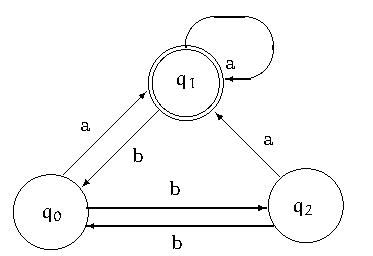
\includegraphics[scale=1]{14ottobre01.pdf}
\end{center}

\noindent $q_1$ è lo stato finale (lo stato finale si indica con un cerchio interno a quello dello stato).

\subsection*{Linguaggio accettato da un automa M}
Definiamo in modo induttivo, a partire dalla funzione $\delta$, la seguente funzione:
\begin{center}
$\hat{\delta}: Q$ x $\Sigma^* \rightarrow Q = $
$\begin{cases} 
\hat{\delta}(q, \varepsilon) = q & $ se la stringa è vuota, resto nello stato$\\
\hat{\delta}(q, wa) = \delta(\hat{\delta}(q, w), a)
\end{cases} $
\end{center}

\noindent Allora un linguaggio accettato da un automa $M$ è:
\begin{center}
$\mathfrak{L}(M) = \{ \sigma \in \Sigma^* $ | $ \hat{\delta}(q_0, \sigma) \in F\}$  
\end{center}

\noindent I linguaggi $\mathfrak{L} \in \Sigma^*$ accettati da un automa a stati finiti sono detti \textbf{regolari}.\\

Attenzione: per ogni linguaggio regolare esistono infiniti grafi a stati finiti.\\

\newpage

\noindent \underline{Esempio 1}:\\

\begin{center}
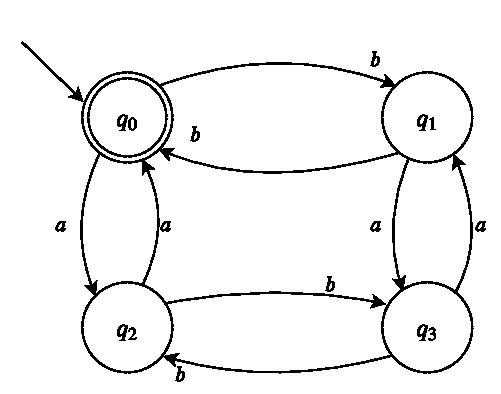
\includegraphics[scale=0.8]{14ottobre02.pdf}
\end{center}

\noindent Il seguente automa accetta solo stringhe che:
\begin{itemize}
\item[-] Hanno numero pari di $a$ (se è presente questo simbolo nella stringa);
\item[-] Hanno numero pari di $b$ (se è presente questo simbolo nella stringa);
\end{itemize}

\noindent Infatti la stringa $ababb$ non è accettata.

\begin{tcolorbox}
Come costruire un grafo: Per capire di quanti stati necessita un grafo, bisogna tenere a mente/definire il significato di ogni stato.

Dall'esempio sopra:
\begin{itemize}
\item[-] $q_1$ -> $a$ pari, $b$ dispari;
\item[-] $q_2$ -> $a$ dispari, $b$ pari;
\item[-] $q_3$ -> $a$ dispari, $b$ dispari;
\end{itemize}
\end{tcolorbox}

\noindent \\ \underline{Esempio 2}:\\

\begin{center}
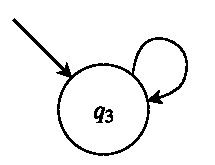
\includegraphics[scale=1]{14ottobre04.pdf}
\end{center}

\noindent L'unico linguaggio accettato dal seguente automa è rappresentato dall'insieme vuoto.

\noindent \\ \underline{Esempio 3}:\\

\begin{center}
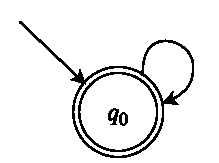
\includegraphics[scale=1]{14ottobre03.pdf}
\end{center}

\noindent Il seguente automa accetta tutte le stringhe -> $\{a, b\}^*$.

\subsubsection*{Esercizio}

Dato il seguente linguaggio, con relatico alfabeto, determinare la macchina a stati finiti deterministica associata e dimostrare è corretta:\\

$\Sigma = \{0, 1\}$ \hspace{1cm} $\mathfrak{L} = \{ x \in \Sigma^*$ | in x occorre almeno uno 0$\}$\\
 
\noindent Possibilità 1

\begin{center}
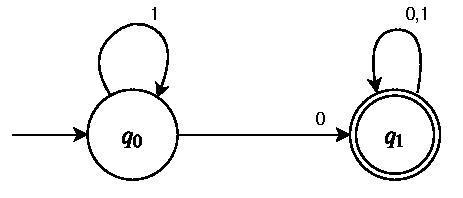
\includegraphics[scale=1]{14ottobre05.pdf}
\end{center}

\noindent Possibilità 2

\begin{center}
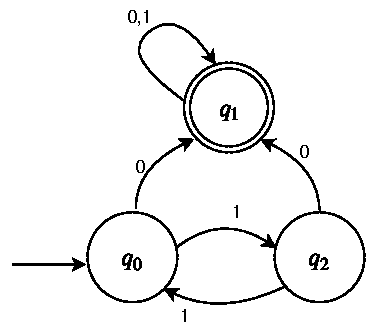
\includegraphics[scale=1]{14ottobre06.pdf}
\end{center}

\noindent Osservazioni: 
\begin{itemize}
\item[-] $q_0$ rappresenta lo stato in la stringa non appartiene al linguaggio;
\item[-] $q_1$ rappresenta lo stato in la stringa appartiene al linguaggio;
\item[-] La stringa vuota non appartiene al linguaggio (non contiene 0);
\end{itemize}

\noindent Dimostrazione della correttezza della possibilità 1:

\subsection*{Problema decisionale}
Finita la lettura di tutta la stringa, la macchina ritorna un si se l'automa si trova in uno degli stati finali, altrimenti no.

\end{document}